 

\section{TCP}
\problem{}
\begin{figure}	
\end{figure}

\begin{align*}
	&\text{IP: } 192.168.1.102 \\
	&\text{Port: } 1161
\end{align*}

{
\centering
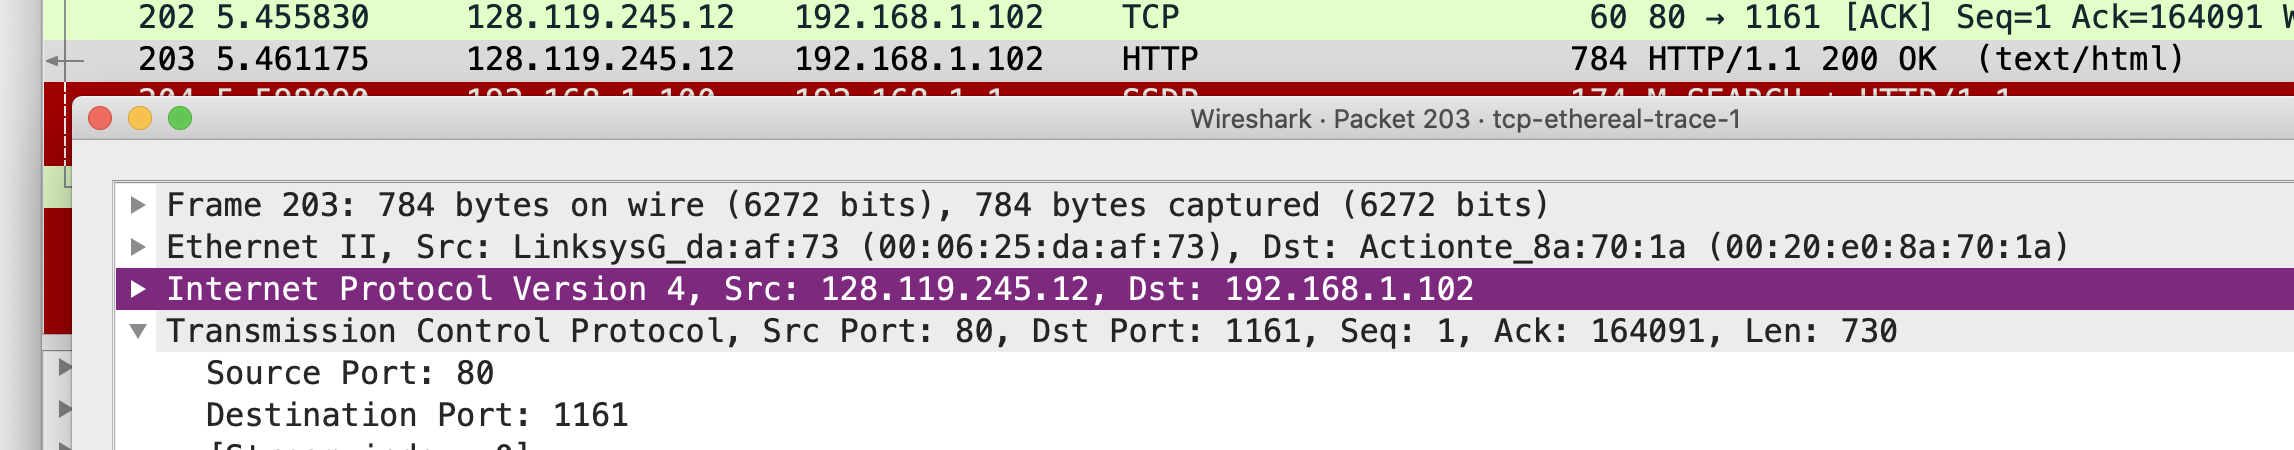
\includegraphics[scale = 0.4]{s1}
}

\problem{}

\begin{align*}
	&\text{IP: } 128.119.245.12 \\
	&\text{Port: } 80
\end{align*}

{
\centering
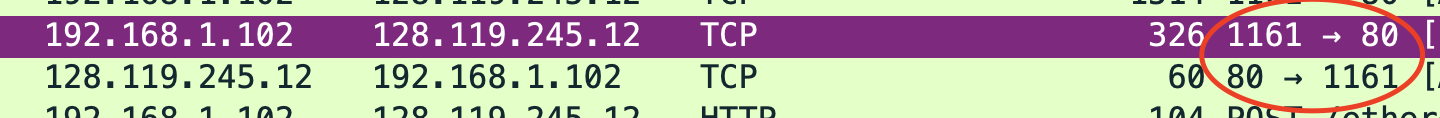
\includegraphics[scale = 0.6]{s2}
}

\problem{}

{
\centering
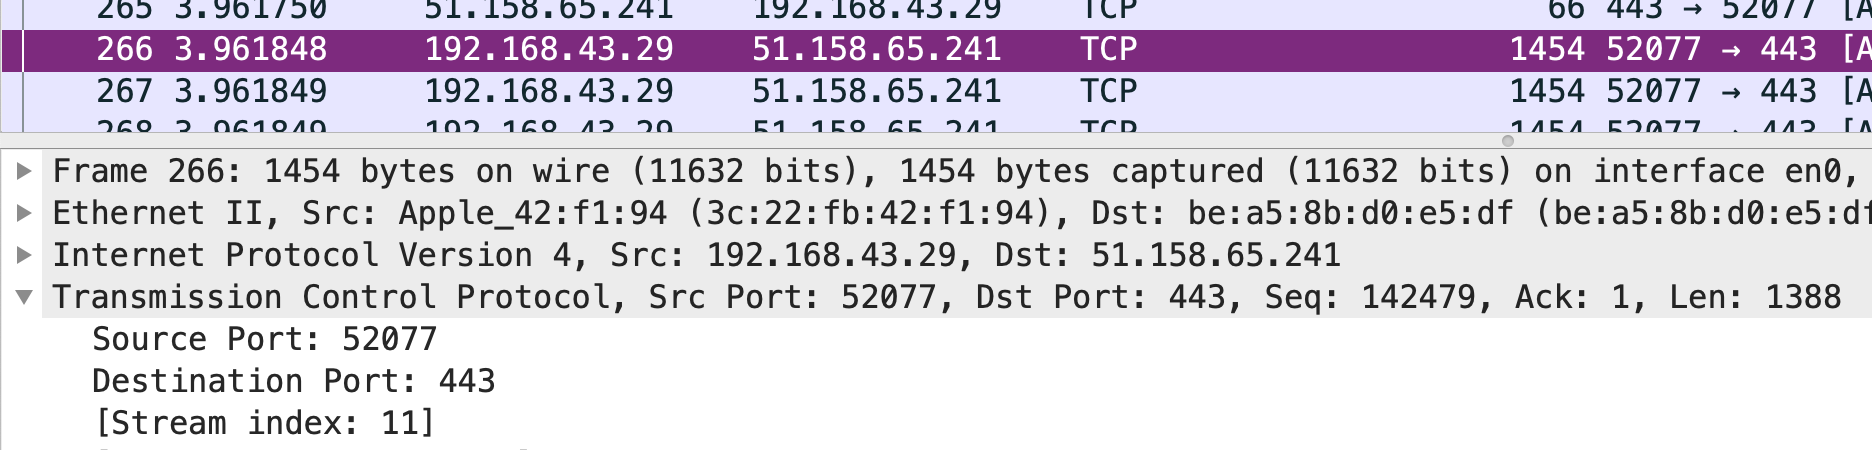
\includegraphics[scale = 0.50]{s3}
}

\begin{align*}
	&\text{IP: } 192.168.43.29 \\
	&\text{Port: } 52077
\end{align*}

\problem{}

{
\centering
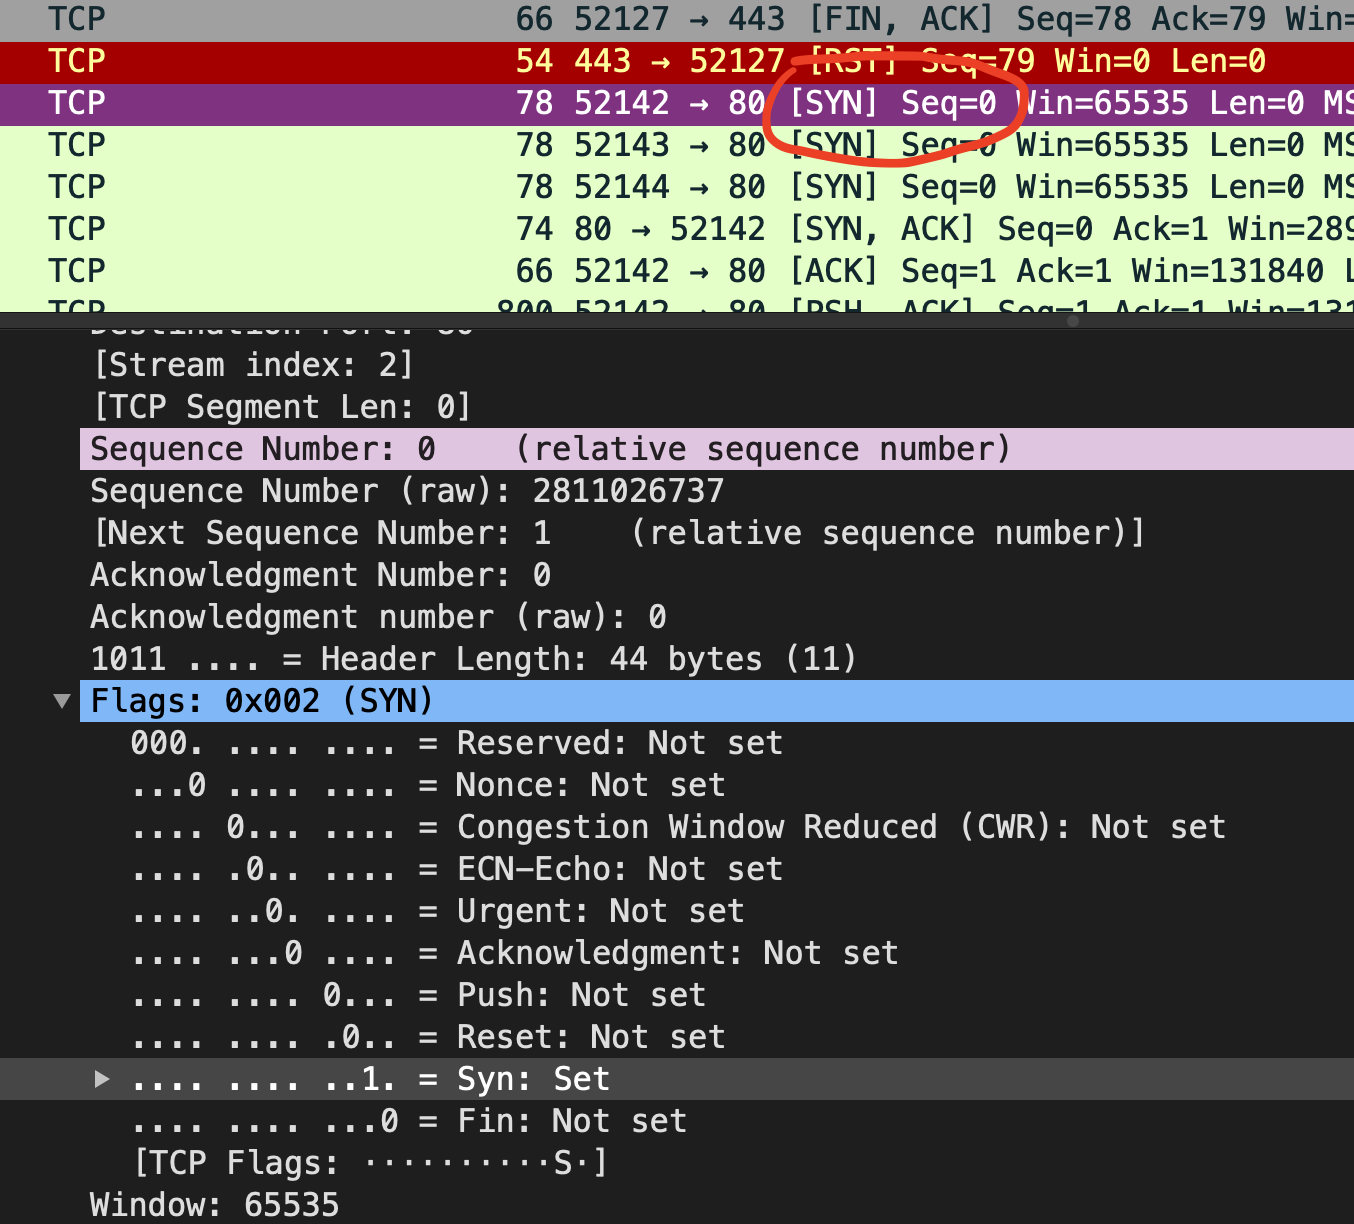
\includegraphics[scale = 0.65]{s4} \\
\begin{latin}
a) sequence number = 0 \\
b) the sequence number being zero and the syn flag being set.
\end{latin}
}

\problem{}
{
\centering
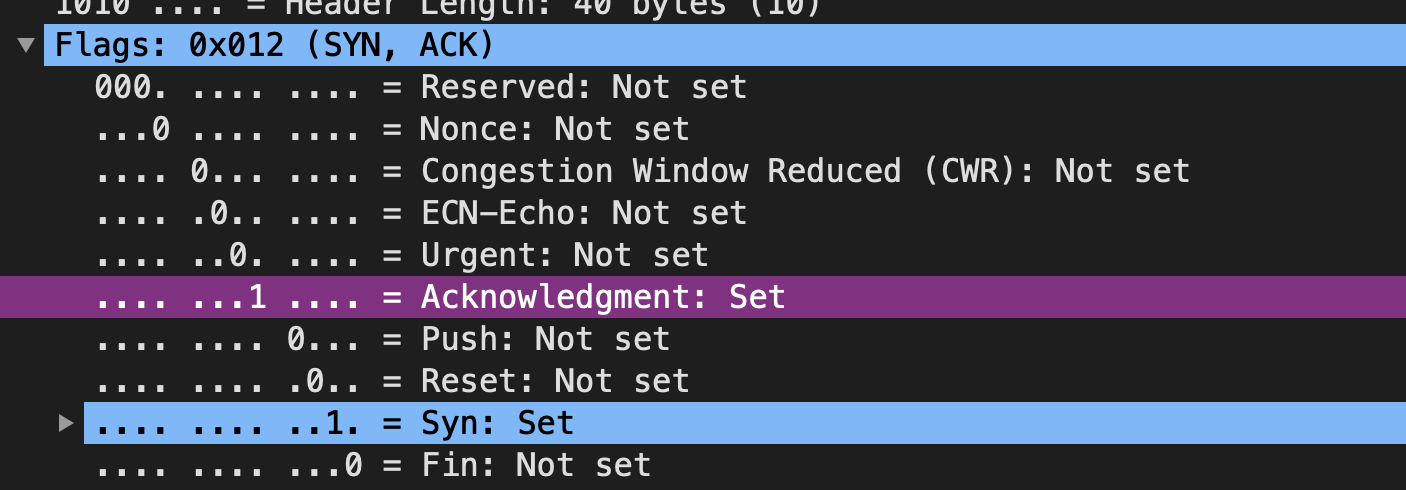
\includegraphics[scale = 0.65]{s5} \\
\begin{latin}
(check previous figure) the sequence number is 0 in response to syn segment). \\
the value of acknowledgement field in synack is 1 (1+ sender sequence number). \\
the syn and ack fields being set to 1.
\end{latin}
}

\problem{}

{
\centering
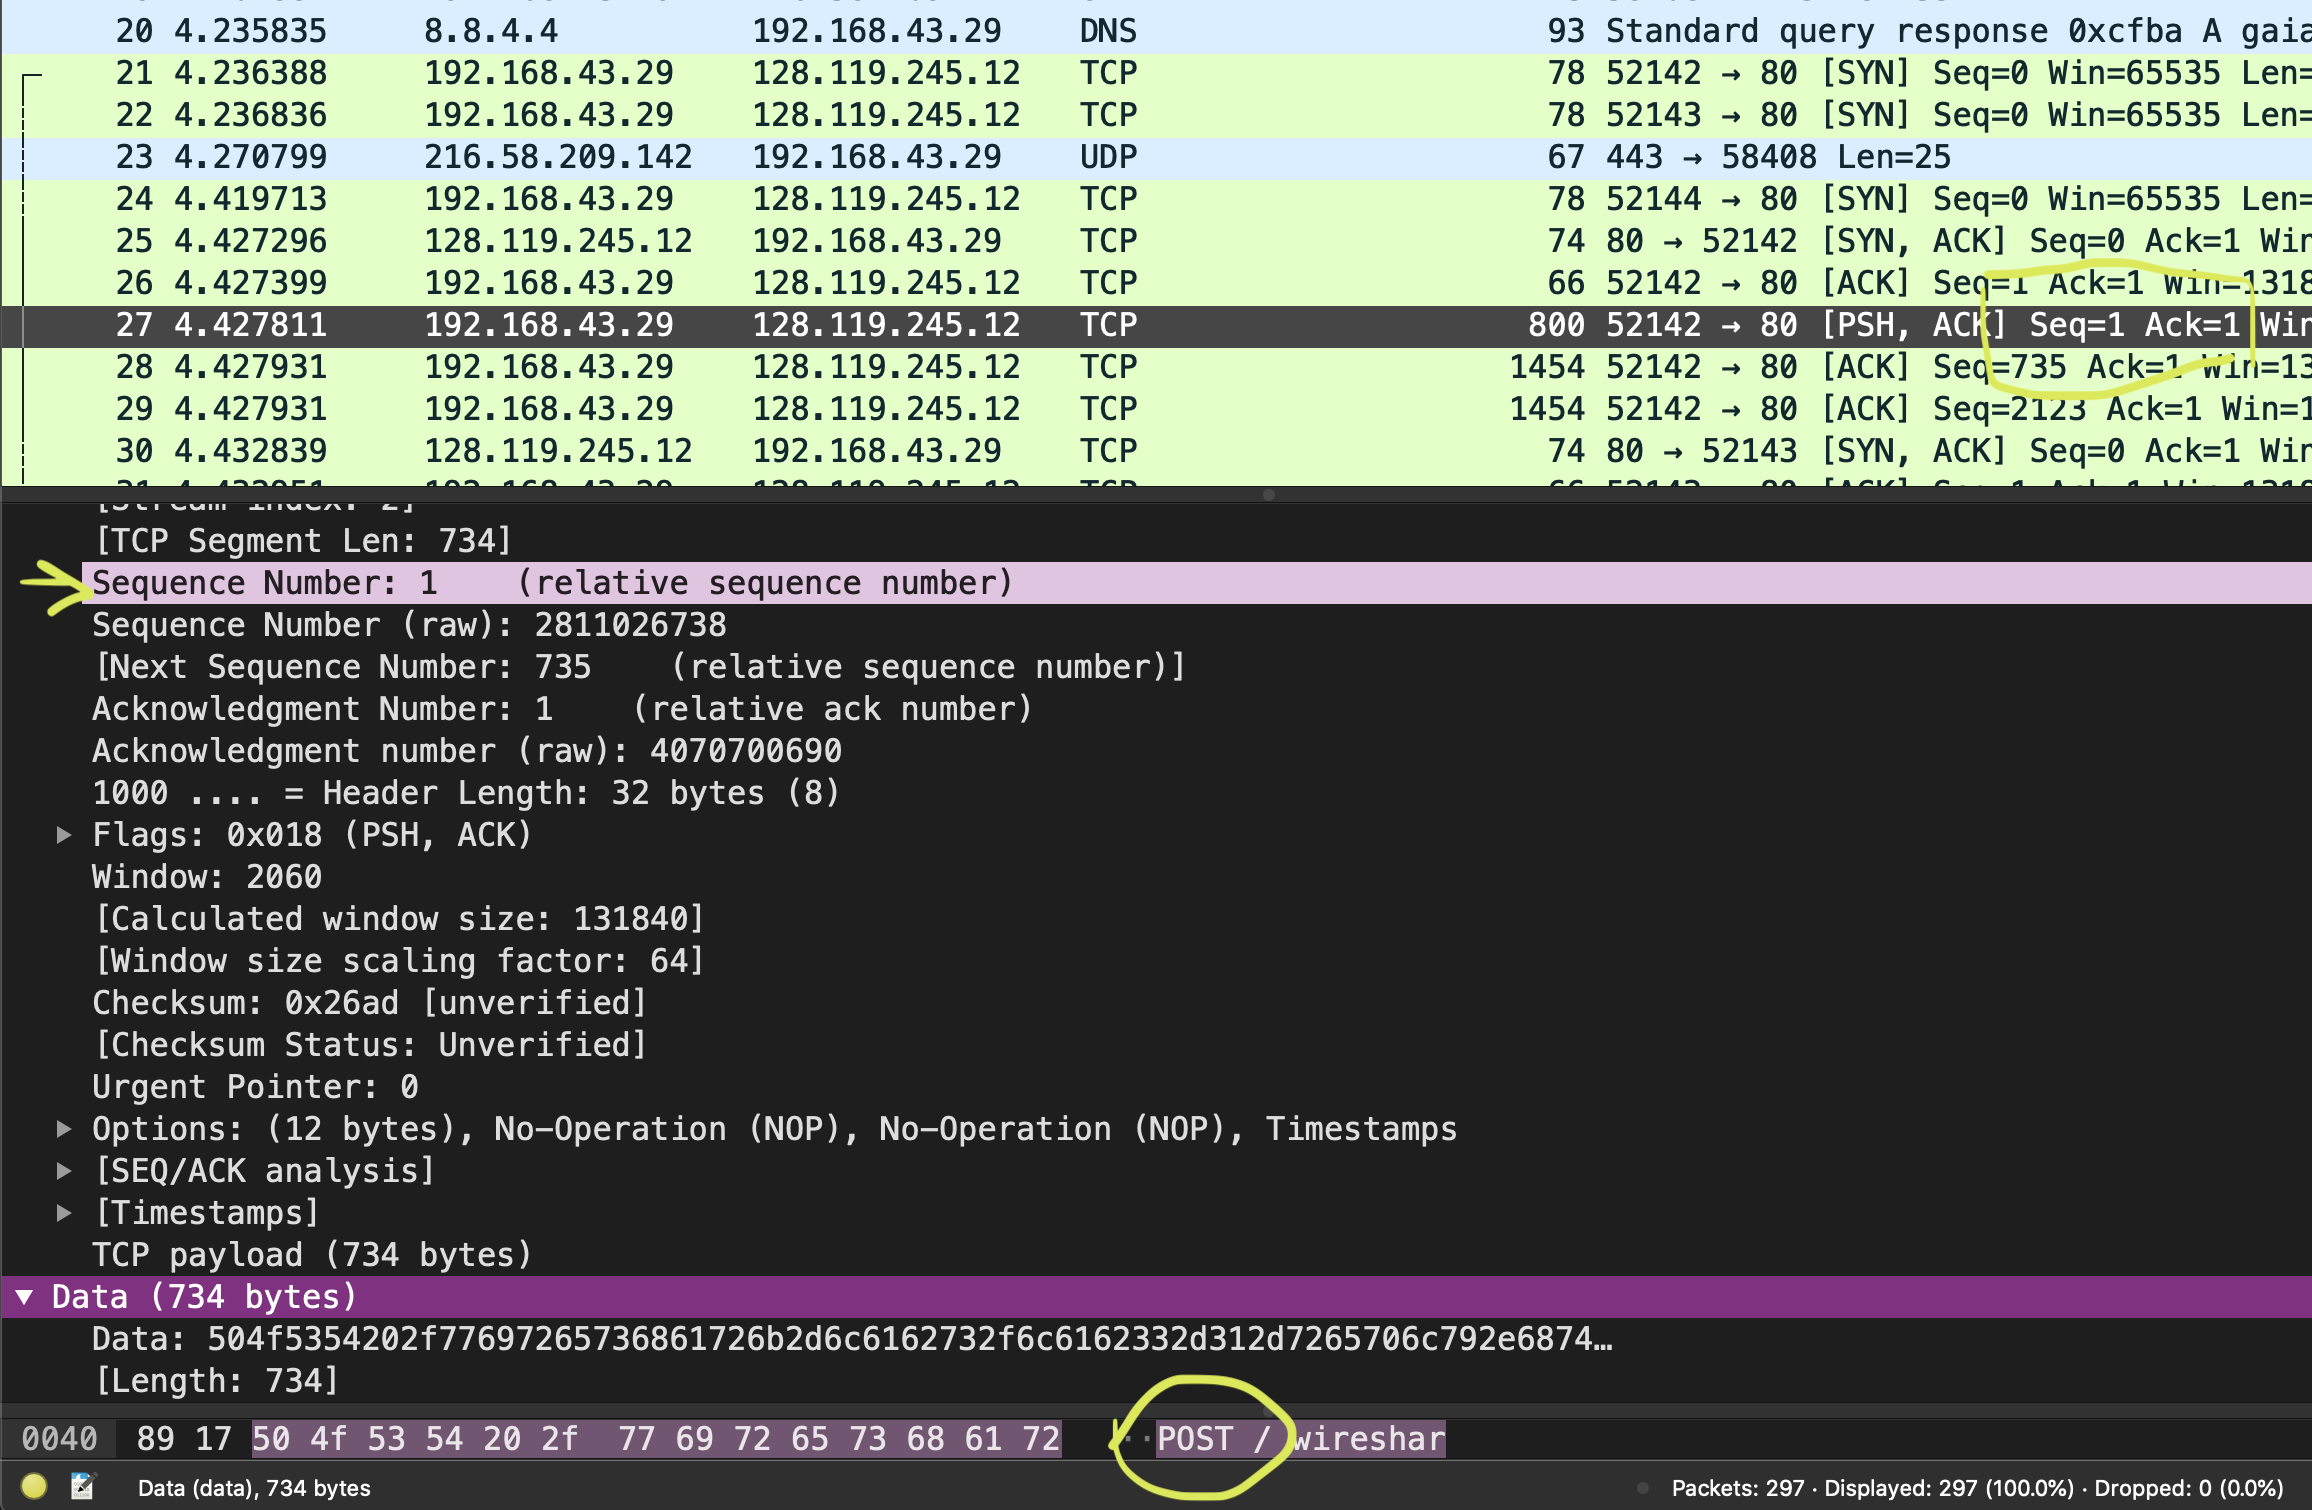
\includegraphics[scale = 0.39]{s6.png}} \\
\begin{latin}
a) sequence number = 1	
\end{latin}
}


\problem{}
\begin{equation*}
	\text{ظرفیت لینک }= 4 \unit{ Mb/s} * \frac{1 \unit{ MB}}{8 \unit{ Mb}} = 500 \unit{ Kb/s}
\end{equation*}

\subproblem{}

\begin{equation*}
	500 \unit{ Kb/s} \div 25 \unit{ Kb/s} = 20 \unit { نفر}
\end{equation*}


\subproblem{}

\begin{equation*}
	P [X > N] = 1 - P [X \leq N]
\end{equation*}

\begin{equation*}
	P [X \leq N] = \sum_{x=0}^{N} P[x = N] = \sum_{i=0}^{N} {100 \choose i} p^i (1-p)^{100-i}
\end{equation*}

و داریم 
$p = 10\% = 0.1$
.	 
پس

\begin{equation*}
	P [X \leq N] = \sum_{i=0}^{N} {100 \choose i} (0.1)^i (0.9)^{100-i} = (0.1)^{100} \sum_{i=0}^{N} {100 \choose i} 9^{100-i}
\end{equation*}
	
که شکل باز شده آن این گونه خواهد بود:

\begin{equation*}
	P [X \leq N] = 0.9^{100} * [1 + 100/9 + 10000/18 + ...]
\end{equation*}

در نهایت داریم:

\begin{equation*}
	P [X > N] = 1 - 0.1^{100} \sum_{i=0}^{N} {100 \choose i} 9^{100-i} 
\end{equation*}

\subproblem{}
در روش 
\lr{circuit swtching}
این مزیت وجود دارد که بسته ما بدون نیاز به این 
که منتظر بسته‌های غیرمرتبط دیگر بماند به سمت مقصد می‌رود.
این ویژگی باعث می‌شود برای کارهای
\lr{real time}
مثل تماس‌ صوتی یا تصویری
گزینه‌ای مناسب باشد
.

از طرفی رزرو (اشغال) بودن لینک به آن معنا است که اگر دو کابری که به هم متصل شده‌اند برای مدتی اطلاعاتی
رد و بدل نکنند٫ لینک بین آن‌ها 
\lr{idle}
باقی میماند و از آن پهنای باند استفاده مفید دیگری نمی‌شود. 

در روش 
\lr{packet switching}
از طرفی می‌توان در هر لحظه از کل پهنای باند در دسترس استفاده کرد. در نتیجه اگر شبکه ما تعداد کاربر زیادی نداشته باشد یا تعداد زیادی در آن واحد از آن استفاده فعال نکنند٫
در عمل مانند 
\lr{circuit switching}
عمل می‌کند٫ بدون آن که هزینه‌های آن را پرداخت کرده باشد.
و تعداد کاربرهای بیشتری را در  پهنای باند مشابه پشتیبانی می‌کند.


همان‌طور که اشاره شد در روش circuit switching خود رزرو کردن لینک و هماهنگ کردن مبدا و مقصد هزینه‌بر و هم به زمان مورد نیاز برای انتقال داده و هم به پیچیدگی شبکه می‌افزاید. در حالی که 
\lr{packet switching}
به نسبت ساده‌تر و کم هزینه‌تر است.

و در نهایت بزرگ‌‌‌ترین بدی 
\lr{packet switching}
(و شاید تنها بدی آن به نسبت)
این است که عملکرد آن با توجه به 
\lr{congestion} 
شبکه می‌تواند متفاوت باشد و در ارتباط
\lr{delay}
وجود خواهد داشت و 
\lr{best effort}
بودن 
\lr{ip‌}
و عبور 
\lr{packet}
ها از مسیرهای مختلف
باعث می‌شود ترتیب رسیدن آن‌ها
(و یا حتی رسیدن آن‌ها)
تضمین نشود
.


